\subsection{Equações}



Após apresentar uma equação, por exemplo, 
\begin{equation} \label{eq:sample}
\frac{\partial F}{\partial t} = \frac{D \partial^2 F}{\partial x^2}, 
\end{equation}
algumas palavras podem ser necessárias para descrever a equação~\eqref{eq:sample},
se houver tempo e espaço suficientes. 

% Some words might be appropriate describing equation~(\ref{eq:sample}), if https://agscan365.sharepoint.com/:f:/g/IgDpUM_6GuCnSLbDp7bUQLXbAcRXGJ7ScpHxyfDrlNy0ER0?e=e7MFAG
% we had but time and space enough. 

Veja \cite{Abl:56}, \cite{AbTaRu:54}, \cite{Keo:58} e \cite{Pow:85}. 

\subsubsection{Exemplo.} 

Esta equação vai muito além do celebrado teorema do grande Pitágoras.

% This equation goes far beyond the
% celebrated theorem ascribed to the great Pythagoras by his followers.
Alguns ambientes como teorema, lema, corolário e prova estão definidos no preâmbulo 
do arquivo {\tt sbaconf.tex}. Por exemplo, para inserir um lema, utilize
\if\portugues1
\begin{verbatim}
\begin{lema}
O quadrado da hipotenusa é igual à soma dos 
quadrados dos catetos em um triângulo retângulo.
\end{lema}
\end{verbatim}
resultando em
\begin{lema}   % use the thm environment for theorems
	O quadrado da hipotenusa é igual à soma dos quadrados dos catetos em um triângulo retângulo. 
% The square of the length of the hypotenuse of a right triangle equals
% the sum of the squares of the lengths of the other two sides.
\end{lema}
\else
\begin{verbatim}
\begin{lem}
O quadrado da hipotenusa é igual à soma dos 
quadrados dos catetos em um triângulo retângulo.
\end{lem}
\end{verbatim}
resultando em
\begin{lem}   % use the thm environment for theorems
	O quadrado da hipotenusa é igual à soma dos quadrados dos catetos em um triângulo retângulo. 
% The square of the length of the hypotenuse of a right triangle equals
% the sum of the squares of the lengths of the other two sides.
\end{lem}
\fi

Para inserir uma prova, utilize
\if\portugues1
\begin{verbatim}
\begin{prova}
Em um triângulo retângulo, a soma do quadrado 
dos catetos (lados menores) é igual ao quadrado 
da bipotenusa (lado maior). 
\end{prova}
\end{verbatim}
resultando em

\begin{prova}    % and the pf environment for proofs
Em um triângulo retângulo, a soma do quadrado dos catetos (lados menores) é igual ao quadrado da bipotenusa (lado maior). 
\end{prova}
\else
\begin{verbatim}
\begin{pf}
Em um triângulo retângulo, a soma do quadrado 
dos catetos (lados menores) é igual ao quadrado 
da bipotenusa (lado maior). 
\end{pf}
\end{verbatim}
resultando em

\begin{pf}    % and the pf environment for proofs
Em um triângulo retângulo, a soma do quadrado dos catetos (lados menores) é igual ao quadrado da bipotenusa (lado maior). 
\end{pf}
\fi

Caso queira criar um novo ambiente, por exemplo, definição, siga o modelo dos ambientes 
criados previamente.

%% There are a number of predefined theorem-like environments in
%% ifacconf.cls:
%%
%% \begin{thm} ... \end{thm}            % Theorem
%% \begin{lem} ... \end{lem}            % Lemma
%% \begin{claim} ... \end{claim}        % Claim
%% \begin{conj} ... \end{conj}          % Conjecture
%% \begin{cor} ... \end{cor}            % Corollary
%% \begin{fact} ... \end{fact}          % Fact
%% \begin{hypo} ... \end{hypo}          % Hypothesis
%% \begin{prop} ... \end{prop}          % Proposition
%% \begin{crit} ... \end{crit}          % Criterion

%Of course LaTeX manages equations through built-in macros. You may
%wish to use the \texttt{amstex} package for enhanced math
%capabilities.

É claro, todos os recursos do {\LaTeX} para o tratamento de equações podem
ser utilizados para melhorar a apresentação. 

\subsection{Figuras}

Para inserir figuras, use o pacote \texttt{graphicx}. Outros pacotes podem
também ser usados, porém  \texttt{graphicx} é um dos mais simples. Veja
a Figura~\ref{fig:bifurcation} como exemplo. 

%To insert figures, use the \texttt{graphicx} package. Although other
%graphics packages can also be used, \texttt{graphicx} is simpler to
%use. See  Fig.~\ref{fig:bifurcation} for an example.

\begin{figure}
\begin{center}
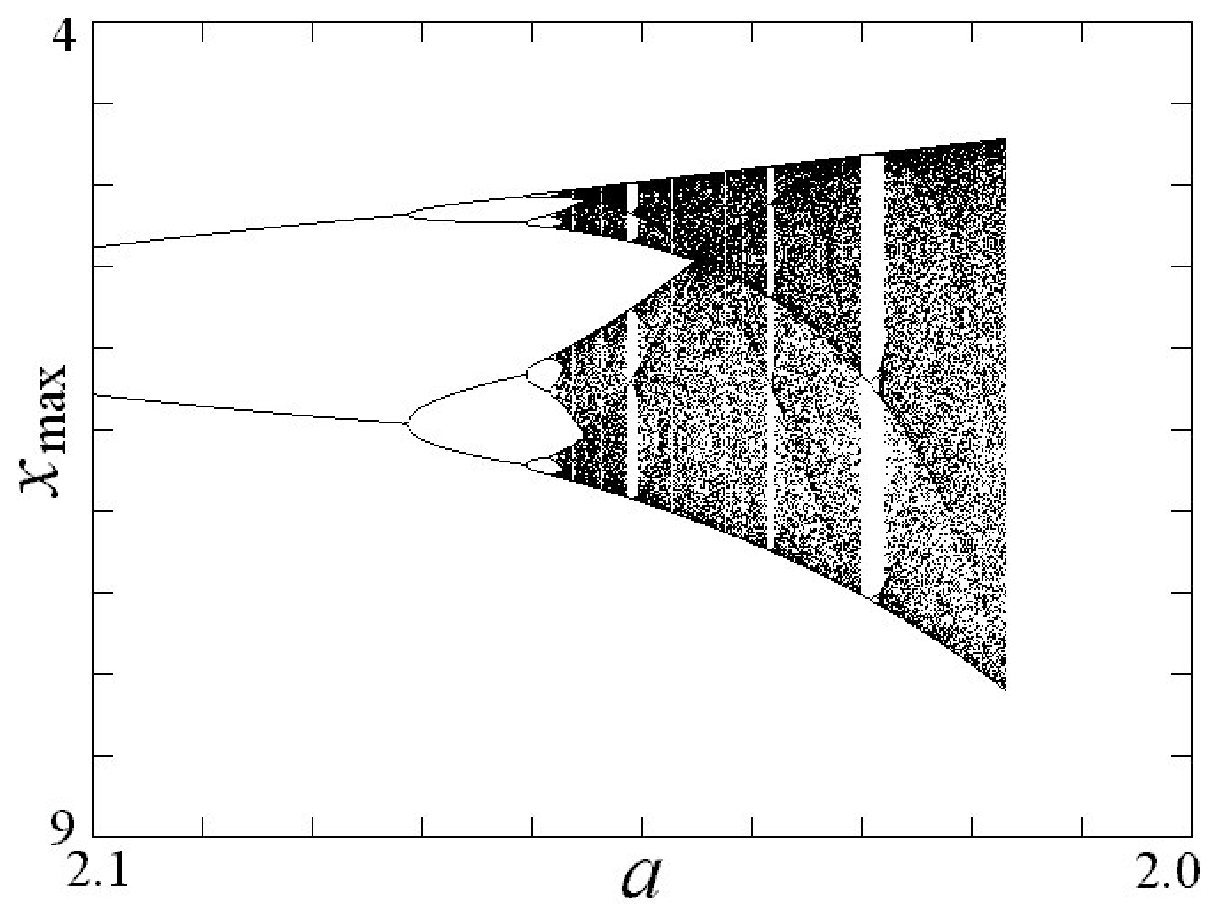
\includegraphics[width=8.4cm]{bifurcation.eps}    % The printed column width is 8.4 cm.
\caption{Bifurcação: Máximos locais de $x$ com o amortecimento $a$ decrescendo.} 
\label{fig:bifurcation}
\end{center}
\end{figure}

Figuras devem ser centralizadas, e ter uma legenda abaixo. 
% Figures must be centered, and have a caption at the bottom. 

\subsection{Tabelas}

Tabelas devem ser centralizadas, ter uma legenda acima e ser numeradas em arábicos.
Veja a Tabela~\ref{tb:margins} para um exemplo. 

%Tables must be centered and have a caption above them, numbered with
%Arabic numerals. See table~\ref{tb:margins} for an example.

\begin{table}[hb]
\begin{center}
\caption{Margens.}\label{tb:margins}
\begin{tabular}{cccc}
Página & Topo & Baixo & Esquerda/Direita \\\hline
Primeira & 3,5 & 2,5 & 1,5 \\
Demais & 2,5 & 2,5 & 1,5 \\ \hline
\end{tabular}
\end{center}
\end{table}